\chapter{Methodology}
\label{methodology}

In order to fulfil the goal of this thesis, it is important to first investigate which steps are necessaryto take towards the results. Once these steps are known, different methodological approaches must be analyzed and compared.

In this chapter, we will firstly pass through a simple illustrative example with the goal of providing the reader a better overview of the domain and explaining the idea behind getting log messages into more organized structures. After that, we include a detailed description of the proposed approaches on developing a machine learning based anomaly detection tool. 

\section{Overview of the Proposed Approach}
The goal of our approach is to fulfil the objective of the thesis and answer the research questions listed in Chapter \ref{introduction}. The final step that needs to be conducted is trivially, applying anomaly detection methods. As a matter of fact, our dataset is mostly unlabeled, thus we need to exploit unsupervised anomaly detection methods aided by unlabeled data. However, the main focus of the methodological approach of our research is on the preprocessing steps that lead to the final machine learning application. Figure \ref{fig:worklowOverview} shows the pipeline of the key steps employed in this study. Despite the simple structure of the workflow pipeline, in reality, the process gets much more complex and requires several back and forth iterations, due to some inconsistencies in datasets, new findings from observing the data, etc.

Because we are using a real-world dataset, we needed to familiarise ourselves with the domain, choose some specific parts the log data valid for our research and then investigate, what characteristic properties could be extracted from the log data that would reflect the underlying events. Given the importance of data processing to be done correctly, it is further structured into three phases.

As a first step, it is necessary to collect the log data from the monitored system. We will examine several possibilities of gathering data from SmartConnect's system and explain which one did we choose and why. We show how those logs are parsed and event types are mined from raw log messages. We proceed with a discussion on feature engineering and how we apply windowing on the time series data. After that, we explain how we applied the selected machine learning algorithms on the preprocessed data. 

To conclude, the following four steps of our solution will be described more comprehensively in the remainder of this chapter.

\begin{enumerate}
    \item Data Collection 
    \item Log Parsing
    \item Feature Engineering
    \item Anomaly Detection
\end{enumerate}

\begin{figure}[h]
    \centering
    
\begin{tikzpicture} [
    edge/.style={-latex,shorten >=1pt, thin, color=customGrey},
    line/.style={-,shorten >=1pt, thin, color=customGrey},
    mainRectangle/.style={rectangle, draw=customBlue, align=center},
    dataCollectionCylinder/.style={cylinder, draw=customBlue, shape aspect = 0.3, align=center, shape border rotate=90}
]
    % DATA COLLECTION
    \node[mainRectangle, minimum width={40mm}, label={[label distance=2mm, align=center]{ \footnotesize 1. Data collection}}] (dataCollection) at (0, 0) {
        \begin{tikzpicture}[node distance=1cm,outer sep=0pt]
          \node[dataCollectionCylinder, minimum width={25mm}, minimum height={10mm}] (dataCylinder) {\scriptsize Log file};
        \end{tikzpicture}
    };
    
    % LOG PARSING
    \node[mainRectangle, minimum width={43mm},
    label={[label distance=2mm, align=center]{\footnotesize 2. Log parsing}}] (logParsing) at (6, 0) {
        \begin{tikzpicture}[align=center]
            \node[mainRectangle, densely dashed, minimum width={30mm}, label={[label distance=0mm, align=center]{\scriptsize Template mining}}] (templateMining) {
                \begin{tikzpicture}
                    \node[rectangle, draw=customDarkRed, align=center, solid] (rawLog) at (6, -2) {\textcolor{customDarkRed}{\tiny RAW LOG}};
                    \node[rectangle, draw=customDarkRed, align=center, solid] (eventTemplate) at (6, -4) {\textcolor{customDarkRed}{\tiny LOG EVENT}};
                    \draw[edge, solid] (rawLog) -- (eventTemplate);
                \end{tikzpicture}
            };
        \end{tikzpicture}
    };
    \draw[edge] (dataCollection) -- (logParsing);
    
    % FEATURE ENGINEERING
    \node[mainRectangle, minimum width={50mm},
    label={[label distance=2mm, align=center]{\footnotesize 3. Feature engineering}}] (featureEngineering) at (6,-6) {
        \begin{tikzpicture}[node distance=1cm,outer sep=0pt]
        % WINDOWING
            \node[mainRectangle, align=center, densely dashed, minimum width={30mm}, label={[label distance=0mm, align=center]{\scriptsize Windowing}}] (windowing) {
                \begin{tikzpicture}
                    % LOG EVENTS
                    \node[rectangle, draw=customDarkRed, fill=white, align=center, solid] (logEventWindow3) at (6.2, -3.8) {\textcolor{customDarkRed}{\tiny LOG EVENT}}; 
                    \node[rectangle, draw=customDarkRed, fill=white, align=center, solid] (logEventWindow2) at (6.1, -3.9) {\textcolor{customDarkRed}{\tiny LOG EVENT}}; 
                    \node[rectangle, draw=customDarkRed, fill=white, align=center, solid] (logEventWindow1) at (6, -4) {\textcolor{customDarkRed}{\tiny LOG EVENT}};
                    
                    % LOG SEQUENCE
                    \node[rectangle, draw=customDarkRed, align=center, solid] (logSequence) at (6, -6) {\textcolor{customDarkRed}{\tiny LOG SEQUENCE}};
                    
                    \draw[edge, solid] (logEventWindow1) -- (logSequence);
                \end{tikzpicture}
            };
            
            % FEATURE VECTOR EXTRACTION
            \node[mainRectangle, align=center, densely dashed, minimum width={30mm}, label={[label distance=0mm, align=center]{\scriptsize Feature vector extraction}}] (featureVectorExtraction) at (0,-3) {
                
                \begin{tikzpicture}
                    \node[rectangle, draw=customDarkRed, align=center, solid, minimum width={15mm}] (eventCountVector) at (0, 0) {\textcolor{customDarkRed}{\tiny EVENT COUNT}\\\textcolor{customDarkRed}{\tiny VECTOR}};
                    
                    \node[rectangle, draw=customDarkRed, align=center, solid, minimum width={15mm}] at (2, 0) (tfIdfVector) {\textcolor{customDarkRed}{\tiny TF-IDF}\\\textcolor{customDarkRed}{\tiny VECTOR}};
                \end{tikzpicture} 
            };
            
            \draw[line, solid] (windowing) -- (0, -2);
            \draw[edge, solid] (0, -2) -| (-2.3, -2) |- (-1.95, -3);
            \draw[edge, solid] (0, -2) -| (2.3, -2) |- (1.85, -3);
        \end{tikzpicture}
    };
    
    \draw[edge] (node cs:name=logParsing, anchor=east) -| (9, 0) |- (node cs:name=featureEngineering, anchor=east);
    
    \node[mainRectangle, minimum width={40mm}, label={[label distance=2mm, align=center]{ \footnotesize 4. Anomaly Detection}}] (anomalyDetection) at (0, -6) {
        % FEATURE MATRIX
        \begin{tikzpicture}
            \node[rectangle, draw=customDarkRed, align=center, solid, minimum width={30mm}] (featureMatrix) at (0, -2) {\textcolor{customDarkRed}{\tiny FEATURE MATRIX}};
            
            \draw[edge, solid] (featureMatrix) -- (0, -3);
            \draw[edge, solid] (featureMatrix) -- (-1.4, -3);
            \draw[edge, solid] (featureMatrix) -- (1.4, -3);
        
         % ML METHODS
        \node[mainRectangle, align=center, densely dashed, minimum width={30mm}, label={[label distance=0mm, align=center]{\scriptsize ML Methods}}] (mlMethods) at (0,-4) {
            \begin{tikzpicture}
                \node[rectangle, draw=customDarkBlue, align=center, solid, minimum width={10mm}] (pca) at (0, 0) {\textcolor{customDarkBlue}{\tiny PCA}};
                
                \node[rectangle, draw=customDarkBlue, align=center, solid, minimum width={13mm}] at (1.4, 0) (isolationForest) {\textcolor{customDarkBlue}{\tiny ISOLATION}\\\textcolor{customDarkBlue}{\tiny FOREST}};
                
                \node[rectangle, draw=customDarkBlue, align=center, solid, minimum width={13mm}] at (3.15, 0) (invariantMining) {\textcolor{customDarkBlue}{\tiny INVARIANT}\\\textcolor{customDarkBlue}{\tiny MINING}};
            
            \end{tikzpicture} 
        };
       \end{tikzpicture}
    };
    \draw[edge] (featureEngineering) -- (anomalyDetection);
    
    \node[rectangle, draw=customGreen, align=center, solid, minimum width={10mm}] (result) at (0, -8.4) {\textcolor{customGreen}{\small Anomalies}};
    \draw[edge] (anomalyDetection) -- (result);
    
\end{tikzpicture}


    \caption{The workflow of our anomaly detection solution.}
    \label{fig:worklowOverview}
\end{figure}


\subsection{Toy Example}
To better understand the mathematical modelling and encoding that is required to apply machine learning algorithms for anomaly detection and also to provide a proof of concept, that an anomalous change in logs can indeed be detected, it is nice to have a simple toy scenario. We will simulate a chain of microservices sending traffic from one end to another.

Let's set $m$ as a number of services denoted $s_i$, which are connected in a sequential fashion: $s_0 \rightarrow s_1 \rightarrow s_2 \rightarrow ... \rightarrow s_{m-1}$. Packets are being sent from $s_1$ to $s_m$.

Over the course of $n$ epochs, we send $n$ packets labeled $p_1, p_2, p_3, ..., p_n$ to $s_1$.

At every epoch, a service $s_i$ can execute one of the following simple events: 

\begin{itemize}
    \item $\mathbf{E_1}$: Successfully sent a packet (SEND)
    \item $\mathbf{E_2}$: No packet was sent (FAIL)
\end{itemize}

For each event, we assign a probability of that event happening. For events it holds that 

\begin{gather*}
    Pr[E_1] + Pr[E_2] = 1
\end{gather*}

and each service can have a event different probability distribution.

At every step, every service $s_i$ will log the choice of event for every existing packet denoted as $s_i: p_{j_{E_k}}$. In our simple scenario, the event $E_2:$ FAIL is an anomaly. 

We will construct a machine learning model using supervised learning, logistic regression and decision tree (unlike our actual experiments, where we use strictly only unsupervised learning methods) with the goal of finding out which service failed to send a package. We will run the simulation for $n$ epochs. The prediction $Y$ of our model is either the service that failed, or no service in case of non-anomalous execution. The training set consists of vectors, where each dimension represents a service and the value at each dimension is the event executed by that service in given epoch. 

Firstly, we created a simulation and its illustration can be found in Figure \ref{figure:simulation}. We have given the simulation the following properties: 

\begin{itemize}
    \item Number of services $m = 5$: $s_0 \rightarrow ... \rightarrow s_{4}$
    \item Number of epochs $n = 5000$
    \item Events $E_1$ and $E_2$
    \item Services $s_0, s_1, s_3, s_4$ have a $1\%$ probability of event FAIL and service $s_2$ has a $5\%$ probability of a failure event $E_2$:
    \begin{align*}
        \forall i \in \{0, 1, 3, 4\}: Pr_i[E_1] &= p_i = 0.99 \\
        i = 2: Pr_i[E_1] &= p_i = 0.95
    \end{align*}
\end{itemize}

\begin{figure}\centering
     \begin{tikzpicture}[
    serviceNode/.style={circle,draw=customDarkBlue,fill=white,thick,inner sep=0pt,minimum size=8mm, thin},
    output/.style={circle,draw=black,fill=customGreen,thick,inner sep=0pt,minimum size=8mm},
    hidden/.style={circle,draw=black,fill=customRed,thick,inner sep=0pt,minimum size=8mm},
    function/.style={rectangle,draw=black,fill=customGrey,thick,inner sep=0pt,minimum size=8mm},
    post/.style={thin, -latex, color=customGrey},
    inEdge/.style={-latex,shorten >=1pt, thin,color=customGrey!50}
    ]
		% output invisible node
		\node[draw=none] (pOut) at (9, 3) {};
		
		\node[serviceNode] (s4) at (8, 3) {\tiny $s_4$}
		edge [post] node[auto] {\textcolor{black}{\tiny $p_4$}} (pOut);
		
		\node[serviceNode, label={[label distance=0.5cm,align=center,font=\fontsize{12}{12}\selectfont]\textcolor{customDarkRed}{\tiny FAIL}\\\small $Pi[E_2]=1 - p_i$}] (s3) at (6, 3) {\tiny $s_3$}
		edge [post] node[auto] {\textcolor{black}{\tiny $p_3$}} (s4);
		
		\node[serviceNode] (s2) at (4, 3) {\tiny $s_2$}
		edge [post] node[auto] {\textcolor{black}{\tiny $p_2$}} (s3);
		
		\node[serviceNode] (s1) at (2, 3) {\tiny $s_1$}
		edge [post] node[auto] {\textcolor{black}{\tiny $p_1$}} (s2);
		
		\node[serviceNode,label={[label distance=0.5cm,align=center,font=\fontsize{12}{12}\selectfont]\textcolor{customDarkBlue}{\tiny SEND}\\\small $Pi[E_1]=p_i$}] (s0) at (0, 3){\tiny $s_0$}
		edge [post] node[auto] {\textcolor{black}{\tiny $p_0$}} (s1);
		
		% input invisible node
		\node[draw=none] (p0) at (-2, 3) {}
		edge [inEdge, densely dashed] node[auto] {\textcolor{black}{\footnotesize packet}}  (s0);
\end{tikzpicture}
	\caption{An example of simulation configuration with $5$ services, with each service having its own probability distribution of events $Pr_i$}.
	\label{figure:simulation}
\end{figure}

The simulation generates a log file with log messages printed out by the services. Below we can see some example log message entries in the simulated log file. Packet is sent sequentially between services in increasing order. If the service $i$ fails to send the package to the next service, it logs a message \texttt{No packet was sent} and the packet does not reach any other service $j$ such that $j$ > $i$. Those services also don't record any log message. 

\begin{verbatim}
========== Starting new simulation ==========
Epoch: 0 Service 0: Successfully sent a packet
Epoch: 0 Service 1: Successfully sent a packet
Epoch: 0 Service 2: Successfully sent a packet
Epoch: 0 Service 3: Successfully sent a packet
Epoch: 0 Service 4: Successfully sent a packet
Epoch: 1 Service 0: Successfully sent a packet
Epoch: 1 Service 1: Successfully sent a packet
Epoch: 1 Service 2: No packet was sent
Epoch: 2 Service 0: Successfully sent a packet
Epoch: 2 Service 1: Successfully sent a packet
Epoch: 2 Service 2: Successfully sent a packet
Epoch: 2 Service 3: Successfully sent a packet
Epoch: 2 Service 4: Successfully sent a packet
Epoch: 3 Service 0: Successfully sent a packet
Epoch: 3 Service 1: Successfully sent a packet
Epoch: 3 Service 2: Successfully sent a packet
Epoch: 3 Service 3: Successfully sent a packet
Epoch: 3 Service 4: Successfully sent a packet
Epoch: 4 Service 0: Successfully sent a packet
Epoch: 4 Service 1: Successfully sent a packet
Epoch: 4 Service 2: Successfully sent a packet
Epoch: 4 Service 3: Successfully sent a packet
Epoch: 4 Service 4: Successfully sent a packet
Epoch: 5 Service 0: Successfully sent a packet
Epoch: 5 Service 1: Successfully sent a packet
Epoch: 5 Service 2: Successfully sent a packet
Epoch: 5 Service 3: Successfully sent a packet
Epoch: 5 Service 4: Successfully sent a packet
Epoch: 6 Service 0: Successfully sent a packet
Epoch: 6 Service 1: Successfully sent a packet
Epoch: 6 Service 2: No packet was sent
 \end{verbatim}
 
We can transform the set of log messages into a vector embedding, as can be seen in Table \ref{tab:simulation}. Each row represents one epoch and each cell contains an output of the simulation of a corresponding service, where $1$ is equivalent to event $E_1$ and $0$ is equivalent to event $E_2$. In Figure \ref{fig:simulationPlot} the number of services, that successfully received and sent a packet for each epoch is shown. As expected from the probability distribution of the events, we can see that the majority of epochs finished successfully for all of the $5$ services. Service number $2$ was assigned a higher probability of failure, which corresponds with the number $2$ of successfully executed services on y axes. 

\begin{table}[!h]
\centering
\begin{tabular}{@{}p{1.5cm}p{1.5cm}p{1.5cm}p{1.5cm}p{1.5cm}p{1.5cm}@{}}
\toprule
Epoch      & $\mathbf{s_0}$ & $\mathbf{s_1}$ & $\mathbf{s_2}$ & $\mathbf{s_3}$ & $\mathbf{s_4}$ \\ \toprule
\textbf{0} & 1             & 1             & 1             & 1             & 1             \\
\textbf{1} & 1             & 1             & 0             & 0             & 0             \\
\textbf{2} & 1             & 1             & 1             & 1             & 1             \\
\textbf{3} & 1             & 1             & 1             & 1             & 1             \\
\textbf{4}          & 1             & 1             & 1             & 1             & 1             \\
\textbf{5}          & 1             & 1             & 1             & 1             & 1             \\
\textbf{6}          & 1             & 1             & 1             & 1             & 1             \\ \bottomrule
\end{tabular}
\caption{An example of numerical embedding obtained from the first $7$ epochs of toy example simulation.}\label{tab:simulation}
\end{table}

\begin{figure}[!h]
        \centerline{\includegraphics[scale=.5]{img/dummy_data_plot.pdf}}
        \caption{The result of running our simulation for $5000$ epochs.}
        \label{fig:simulationPlot}
\end{figure}

The obtained simulated dataset can be easily modified to generate labels. If a row is all ones, the assigned label is \texttt{no\_service}. If a row contains a zero, its label is the index of the first service that failed to send a packet. This embedding is then used as an input to create a logistic regression and random forest model. The toy example should provide a better understanding of how can a unstructured textual input be transformed into a format suitable machine learning algorithms.

\section{Data Collection}
\label{data_collection}
By data collection, we understand the process of gathering log data from the observed system in such a way that the logs can be further parsed, processed, and fed to the machine learning model.

The system we study follows the microservices architectural pattern, as described in Section~\ref{smart-connect:architecture} on the architecture of SmartConnect.\\

\subsection{Logging}

Traditionally, an application performs logging by sending messages to
(pseudo) files \texttt{stderr} (standard error) and \texttt{stdout} (standard output). It can be combined with appending those logs also to a dedicated file with \texttt{.log} extension. Both of those practices are usually deployed by services running as containerized applications in Pods\footnote{\url{https://kubernetes.io/docs/concepts/cluster-administration/logging/}}

In the architecture of microservices, this method of logging may not be sufficient,  since a MSA system is usually comprised of many applications and the logs are scattered at many locations. Furthermore, the individual services may be often replaced and contents of log files subsequently removed.

Moreover, in systems that are producing a vast amount of logs, persisting logs in files and stored in service Pod's file system may eventually lead to taking up too much of the node's storage. That's why services such as \texttt{logrotate}\footnote{\url{https://linux.die.net/man/8/logrotate}} are being used. Logrotate collects logs, sends them to a different location, where they can be persisted without affecting MSA system's performance, and removes them from Pod's node. 
On the other hand, this means that when inspecting a Pod, only the most recent (if any) logs can be found in Pod's \texttt{log} file.

When it comes to SmartConnect MSA, an approach similar to the one of \texttt{logrotate}'s is taken.

\texttt{Filebeat}\footnote{\url{https://www.elastic.co/guide/en/beats/filebeat/7.10/filebeat-overview.html}} from ELK (Elasticsearch, Logstash, Kibana)\footnote{\url{https://www.elastic.co/what-is/elk-stack}} is deployed to forward data collected from the system's Pods to Elasticsearch engine (introduced in Section~\ref{smart-connect:elastic-search}). 
The engine represents an authority for storing logs from the system and is considered the single source of truth as the log data is persisted there.

\subsection{Implementation}

To sum up, the following are our options for log collection in the SmartConnect system:
\begin{enumerate}
    \item Saving output of \texttt{kubectl logs \${POD}} command for every relevant Pod
    \item Collecting data saved in \texttt{\${POD}:/var/log/*.log} for each Pod
    \item Requesting logs from SmartConnect's Elasticsearch server
\end{enumerate}

To assess the possibilities, the initial two items represent the same idea, just carried out in a different manner - the \texttt{logs} command just prints the output of the required \texttt{.log} file to \texttt{stdout}. 
It is very easy to get logs of a single Pod, however, to gather all the information we want about the whole system, it requires crawling individually through all of the microservices. Also, as mentioned before, the major drawback of these approaches is that only logs that were not yet picked up by \texttt{filebeat} are accessible.

Therefore, to collect log data from a multiple hours run of the system, it would require to poll the services rather frequently. These methods also bring complexity to data postprocessing, once acquired, as we cannot guarantee uniqueness of entries with these approaches.

On the other hand, the third option is a more difficult one to automate, however promises more structured way of getting the logs. Also, given the features of \texttt{Elasticsearch}, it should also represent faster solution for data collection.

In Motorola, developers review logs stored in their \texttt{Elasticsearch} engine through \texttt{Kibana} web user interface. The UI makes it easy to visualize and filter log data but on the down side, its export options are not well suited for structured way of downloading the data. Regardless of these constraints, there must be a size limit set on the size of the exports. The limit is advised not to be much larger than the default 10MB as it may potentially affect negatively Kibana and Elasticsearch in terms of performance \footnote{\url{https://www.elastic.co/guide/en/kibana/current/reporting-settings-kb.html}}. Speaking in terms of our requirements, 10MB of log data would not span more that a couple of minutes of logs.

Another option, using \texttt{ELK} stack, would be to make use of \texttt{Elasticsearch}'s REST APIs \footnote{\url{https://www.elastic.co/guide/en/elasticsearch/reference/current/rest-apis.html}}. However, for security reasons, some companies may opt out from exposing this API to the internet - Motorola being among them.
The only way to access the application's programming interface is thus to make the calls from inside of the cluster.

We deployed a service called \texttt{elk-query-service} inside of the cluster that handles search requests on the \texttt{Elasticsearch}. Our service exposes a minimalistic functionality that can be accessed within the company.
\texttt{\justify elk-query-service} can be called with two date arguments specifying the start and end of time window. Logs between the start and end date are downloaded to the \texttt{elk-query-service} Pod and can be transferred to the node where they can be further used in a machine learning anomaly detection pipeline as proposed for future work in Section~\ref{future:pipeline}. The high level architecture of our solution for data collection is schematically presented in Figure~\ref{fig:data_collection_elastic}.

\begin{figure}[!tbp] \centering {
   \begin{tikzpicture} [
    edge/.style={-latex,shorten >=1pt, thin, color=customGrey},
    line/.style={-,shorten >=1pt, thin, color=customGrey},
    mainRectangle/.style={rectangle, draw=customBlue, align=left},
]

\node[inner sep=0pt] (mlHost) at (-2,0) {\includegraphics[width=.12\textwidth]{img/computer-icon.png}};
\node[align=center,anchor=north] (lab) at (mlHost.south) {\footnotesize Machine Learning\\\footnotesize Host};
    
\node[mainRectangle, minimum width={20mm}, label={[label distance=2mm]below: \footnotesize MSI Kubernetes Cluster}] (kubernetesCluster) at (4, 0) {
    \begin{tikzpicture}[node distance=1cm,outer sep=0pt, align=left]
        \node[inner sep=0pt, label={[label distance=2mm]below:\footnotesize elk-query-service}] (pod1) at (-2,0)
        {\includegraphics[width=.08\textwidth]{img/pod.png}};   
        
        \node[inner sep=0pt, label={[label distance=2mm]below:\footnotesize elastic-search}] (pod2) at (2,0)
    {\includegraphics[width=.08\textwidth]{img/pod.png}};
    
        \node[draw=none] (a) at (-2.5, 0) {};
        \node[draw=none] (b) at (2.5, 0) {};
        \draw [edge] (a) -- node[anchor=south] {\tiny \textcolor{customDarkRed}{Search Query}} (b);
        \node[draw=none] (c) at (-2.5, -0.3) {};
        \node[draw=none] (d) at (2.5, -0.3) {};
        \draw [edge] (d) -- node[anchor=south] [label=below:\tiny \textcolor{customDarkRed}{Response}]{} (c);
        
        \node[mainRectangle, minimum width={10mm}, label={[label distance=2mm]below: \footnotesize Observed System}] (system) at (0, -3.5) {
            \begin{tikzpicture}[node distance=1cm,outer sep=0pt, align=left]
                \node[inner sep=0pt] (pod3) at (2,0)
                {\includegraphics[width=.06\textwidth]{img/pod.png}};
                \node[inner sep=0pt] (pod4) at (2.8,0)
                {\includegraphics[width=.06\textwidth]{img/pod.png}};
                \node[inner sep=0pt] (pod5) at (3.6,0)
                {\includegraphics[width=.06\textwidth]{img/pod.png}};
                \node[draw=none] (dots) at (4.2, 0) {...};
                \node[inner sep=0pt] (pod3) at (4.8,0)
                {\includegraphics[width=.06\textwidth]{img/pod.png}};
                \node[inner sep=0pt] (pod4) at (5.6,0)
                {\includegraphics[width=.06\textwidth]{img/pod.png}};
                \node[inner sep=0pt] (pod5) at (6.4,0)
                {\includegraphics[width=.06\textwidth]{img/pod.png}};
            \end{tikzpicture} 
        };
        
        \node[draw=none] (es) at (2.2, -1.2) {};
        \node[draw=none] (p1) at (-2.5, -3.3) {};
        \draw [edge] (p1) -- node[anchor=south] {} (es);
        
        \node[draw=none] (p2) at (-1.7, -3.3) {};
        \draw [edge] (p2) -- node[anchor=south] {} (es);
        
        \node[draw=none] (p3) at (-0.9, -3.3) {};
        \draw [edge] (p3) -- node[anchor=south] {} (es);
        
        \node[draw=none] (p4) at (0.4, -3.3) {};
        \draw [edge] (p4) -- node[anchor=south] {} (es);
        
        \node[draw=none] (p5) at (1.3, -3.3) {};
        \draw [edge] (p5) -- node[anchor=south] {} (es);
        
        \node[draw=none] (p6) at (2.15, -3.3) {};
        \draw [edge] (p6) -- node[anchor=south] {} (es);
     
    \end{tikzpicture} 
};
    
    \node[draw=none] (eqs) at (1.6, 2) {};
    \node[draw=none] (mlHostStart1) at (-1.3, 0.8) {};
    \node[draw=none] (mlHostStart2) at (-1.3, 0.5) {};
    \draw [edge] (mlHostStart1) -- node[anchor=south, rotate=22] {\tiny \textcolor{customDarkRed}{Start Date, End Date}} (eqs);
    
    \node[draw=none] (eqs2) at (1.6, 1.7) {};
    \draw [edge] (eqs2) -- node[anchor=north, rotate=22] {\tiny \textcolor{customDarkRed}{Logs}} (mlHostStart2);

\end{tikzpicture}
   \caption{The implemented solution for collecting log data. Node with privileges to access to the Kubernetes cluster calls an orchestrating script with two arguments - start and end date. \texttt{elk-query-service} downloads the desired logs that meet the date requirements. The script stores the response on the machine learning mode that can proceed to next step - training and evaluation of ML models.}
	\label{fig:data_collection_elastic}
	}
\end{figure}

\newpage

\section{Log Parsing}
This section describes our technique for parsing the raw and unstructured logs obtained from the analyzed system.

As pointed out in Section~\ref{log_parsing_techniques} there is many different fundamental approaches to what techniques should be used when extracting message templates from logs. 
Therefore, we developed an extra layer of abstraction over the actual parser that makes our solution less dependent on what specific template mining algorithm is being used.

The experiments therefore work with an object \texttt{LogCategorizer} that exposes functionality to clients. To mention some of the \texttt{LogCategorizer} methods, it provides among others, the following ones:

\begin{itemize}
    \item \texttt{process\textunderscore log\textunderscore message(self, log\textunderscore message: str)\\ -> LogCategory}
    \item \texttt{process\textunderscore log\textunderscore messages(self, log\textunderscore messages: List[str])\\ -> List[LogCategory]}
    \item \texttt{process\textunderscore file(self, input\textunderscore file\textunderscore name: str)}
\end{itemize}

The actual reading and template creating done by these methods is carried out by an instance of \texttt{LogParser}. \texttt{LogParser} is an abstraction - an interface that is used by \texttt{LogCategorizer}. Every implementation of parser needs to fulfill this contract defined by the interface. The interface defines just the bare minimum functionality that is required from a sensible log template miner and that is a pair of methods:
\begin{itemize}
    \item \texttt{get\textunderscore all\textunderscore templates(self) -> List[str]}
    \item \texttt{process\textunderscore log\textunderscore message(self, log\textunderscore message: str) -> str}
\end{itemize}
Therefore an implementation of a log parser should be able to return all the templates that it identified by the moment the \texttt{get\textunderscore all\textunderscore templates} method is called. The other method returns a template based on the raw log message inputed.\\

Our implementation follows the adapter design pattern \cite{gamma1995design_pattern_adapter} as the aim is to convert interfaces of specific log parsing libraries that may be dramatically different in terms of the API that they expose.

This allows us to decouple the implementation of the algorithm that identifies templates from logs from our overall goal and opens the way for easy comparison with different template mining strategies.\\

 \begin{figure}[!h] \centering {
   \resizebox{\textwidth}{!}{
\begin{tikzpicture}

\tikzumlset{draw=customBlue, fill class=white, }

edge/.style={color=black}

\umlclass[x=-9, y=0, width=5ex, name=logCategorizer, text=customDarkRed]{LogCategorizer}{}{
\textcolor{black}{\footnotesize+ try\_insert\_new\_template(template: str)}\\
\footnotesize{+ get\_all\_templates(): [(int, str)]} \\
\footnotesize{+ process\_log\_message(log\_message: str): LogCategory}\\
\footnotesize{+ process\_log\_messages(log\_messages: [str]): [LogCategory]}\\
\footnotesize{+ process\_file(file\_name: str): [LogCategory]}}

\umlclass[x=-9, y=-4, width=5ex, name=logCategory, text=customDarkRed]{LogCategory}{
\textcolor{black}{\footnotesize{+ category\_id: int}}\\
\footnotesize{+ template: str}}{}

\umlclass[x=0, y=0, name=logParser, text=customDarkRed, type=interface]{LogParser}{}{
\textcolor{black}{\footnotesize{+ get\_all\_templates(): [str]}}\\
\footnotesize{+ process\_log\_message(log\_message: str): str}}

\umlclass[x=0, y=-4, name=drain3Parser, text=customDarkRed]{Drain3Parser}{
\textcolor{black}{\footnotesize{- template\_miner: TemplateMiner}}}
{
\textcolor{black}{\footnotesize{+ get\_all\_templates(): [str]}}\\
\footnotesize{+ process\_log\_message(log\_message: str): str}
}

\umlclass[x=0, y=-8, name=templateMiner, text=customDarkRed]{TemplateMiner}
{
\textcolor{black}{\footnotesize{+ clusters}}\\
\footnotesize{+ persistence}}
{
\textcolor{black}{\footnotesize{+ add\_log\_message(log\_message: str)}}
}

\umluniassoc [color=customGrey] {LogCategorizer}{LogCategory}
\umluniassoc [color=customGrey] {LogCategorizer}{LogParser}
\umluniassoc [color=customGrey] {Drain3Parser}{TemplateMiner}
\umldep [color=customGrey] {Drain3Parser}{LogParser}

\end{tikzpicture}
}
   \caption{Architecture for parsing classes. Adapter design pattern application: \texttt{LogParser} as the adapter, \texttt{Drain3Parser} takes on the role of concrete adaptee, \texttt{TemplateMiner} is adaptee - class defined in a different framework with incompatible interface that needs to be converted.}
	\label{fig:uml_parsers}
	}
\end{figure}

In Section~\ref{parser_summary} we mention that our decision was to progress with the framework Drain \cite{drain2017} that performs online fixed-depth tree template mining. The actual implementation of the algorithm we used is \texttt{Drain3} by company IBM\footnote{\url{https://github.com/IBM/Drain3}}. The algorithm follows a template of 5 steps, as described in more depth in Section~\ref{fixed_depth_tree}:
\begin{enumerate}
    \item Preprocess by Domain Knowledge
    \item Search by Log Message Length
    \item Search by Preceding Tokens
    \item Search by Token Similarity
    \item Update the Parse Tree
\end{enumerate}

Let's pay more attention to the first step. It provides us, users, the option to input encoded assumptions and insight on the logs that are produced by the logs.
It is rather intuitive to assume that this domain knowledge, if inserted correctly, should improve the performance and precision of the mining algorithms. An empirical study \cite{he2016} confirms this assumption.
However, we argue that this algorithm tuning technique may not be the option to choose in all use cases. With our solution, we are seeking to analyze a system that is very fluid, therefore likely to change over time. This, together with the fact many developers from multiple teams and companies (taking into account also external software the software system is dependent on), it is unfeasible to maintain a single source of truth regarding domain knowledge related to logging. Conversely, we are aiming for a solution that can learn and adapt to changes as independently as possible.\\

This goal of adaptability is also reflected in the fact that we ended up choosing an online parser.
To remind a definition of an online template miner from Section~\ref{log_template_mining}, an online template miner is such a parser, that does not require to see the whole dataset to start analyzing message templates. It can run categorization on the fly while updating its internal state, which keeps acquired knowledge about the domain.\\
Drain offers the possibility to persist this internal state even between multiple runs, which offers us the best of both worlds - the parser is learning patterns occurring in logs over time to improve while being able to react to new data in flexible fashion.

We have not tweaked steps 2. - 4. as the default parameters \cite{ibmdrain3} yielded results that extracted correct templates from the observed logs.

For the last step, updating the parse tree, Drain3 implementation offers the option to persist the state of the parse tree in JSON file format. This allows us to reuse the  domain knowledge that is acquired by the template miner across restarts of our solution.
This is an extremely useful feature, where we may assume that all of the logs are coming from the same system, we can reuse the parse tree already build in previous runs and enrich it.
Drain3 offers multiple ways of storing the snapshot of parse tree, we are using the one that saves the state into a file.

\section{Feature Engineering}
\label{section:featureEngineering}
Now that we obtained unique event types out of unstructured log messages, we need to choose valuable variables, group them together and encode them into a numerical form that can be further used by the machine learning algorithms. This process is called \textit{feature engineering} or \textit{feature extraction}. Feature extraction is the process of generating new features by doing transformations of the original feature set. On our thesis, we also refer to the generates features as \textit{embeddings}.

Feature engineering step is critically important. Embeddings should be able to summarize valuable information and complex relationships in the dataset, thus directly impacts performance of the learning model, speed of training and avoids overfitting. Log event types generated in the previous step are used as an input for the feature engineering step. The output is a numerical matrix. 

\subsection{Windowing}
% https://core.ac.uk/download/pdf/196555557.pdf page 22

In time-series anomaly detection, a common concept applied in feature extraction is \textit{windowing}. 
Logs are grouped together into smaller blocks called \textit{windows}, where each window represents a sequence of logs. In some previous approaches \cite{xu2009}, they applied windowing by grouping events by the same session identifier, such that each window represents one job execution with an unique identifier. This solution is not be not applicable to our case, as we do not have a session or process id feature in our raw data set.

Log data are also non-evenly spaced time series data, as there is naturally generated a time of occurrence of each log. As a result, another intuitive and frequently used approach to windowing is to generate a set of subsequences of time series. For example, let's say we have log lines ordered by the timestamp and the length of time window is $q$. Then the log line number $1$ to log line number $q$ will be included in the same time window $1$ and encoded as the first row of the resulting feature matrix. The goal of the next anomaly detection step is to tell for each subsequence if it contains an anomaly or not. In our thesis, we use windowing based on timestamp, which is also described in the next part of the text.

Set of time series subsequences can be generated using \textbf{sliding windows}. Let us consider a time series $\mathbf{x} = x_1, x_2, ..., x_n$ of length $n$. We want to extract subsequences $\mathbf{x_i}$ of length $m$. In other words, we want to apply sliding windows of length $m$ and move over the time series until we reach the end of the data set. We shift the window $r$ time steps to the right in each movement. As a result, we get $p$ windows, where $p$ is defined as 
    \begin{gather*}
        p = \dfrac{n - m}{r} + 1
    \end{gather*}

and the generated windows are of form 

\begin{gather*}
    \mathbf{x_1} = x_{11}, x_{12},..., x_{1m} \\
    \mathbf{x_2} = x_{21}, x_{22},..., x_{2m} \\
    \ldots\\
    \mathbf{x_p} = x_{p1}, x_{p2},..., x_{pm} 
\end{gather*}

Size of the step $r$ is a very important parameter. Choosing $r$ to be very low, e.g. $r = 1$ such that subsequences are obtained by sliding window one step at a time, the advantage is that no anomalous sequence can be missed with this approach. However, considering the large data set that grows over time, computations of such subsequences are inefficient and time consuming. On the contrary, we can choose a high value of $r$. For example, if we set $r$ to the length of the sliding window $m$ ($r = m$), then there is no overlap between the windows. The advantage of having a lower number of generated subsequences and decreased processing time comes with a greater risk of missing anomalous subsequences. 

Another parameter to take into consideration, is the size of the sliding window $m$. The ideal size really depends on the application domain and what's the average number of subsequent log entries that can represent an anomaly. 

Thus, setting the size of step parameter $r$ and the length of sliding window $m$ is a trade-off between accuracy and processing time. A useful rule is to choose the value of $r$ proportional to the length of subsequences \cite{izakian2013}. As a result, longer subsequences have higher value of $r$ while shorter subsequences have lower value of $r$. The number of log lines included in each window can vary. 

In our thesis, instead of setting the number of log lines in each window, we consider a size of a subsequence in terms of a time-span.

\begin{figure}[!tbp] \centering {
	\begin{subfigure}[b]{1\textwidth}
        \includegraphics[width=\textwidth]{img/windowing.pdf}		    \caption{Sliding window with a fixed length of $m = 5$ and the size of the step $r = m = 5$}
		\label{fig:f1}
	\end{subfigure} \\
	\hfill
		
    \begin{subfigure}[b]{1\textwidth}
   	    \includegraphics[width=\textwidth]{img/windowing-2.pdf}
		\caption{Sliding window with a fixed length of $m = 10$ and the size of the step $r = 5$}
	\end{subfigure}
	
	\caption{Two types of windowing with different step size $r$. (a) shows sliding windows generated without any overlap. (b) illustrates sliding window generated by stepping half of the window size at the time causing overlaps between subsequent windows.}
	\label{fig:windowing}
	}
\end{figure}

\subsection{Feature embedding}
\label{subsection:features}
After applying the sliding window to generate log sequences, the final step of feature extraction is to construct the feature matrix that can be passed as an input to ML algorithms. In our thesis, we experiment with two different types of embeddings, where both representations describe a group of logs in log sequences: \textit{event count matrix} and \textit{TF-IDF weighted matrix}. Figure \ref{fig:feature-extraction} illustrates an example of a generation process of one single log sequence into a feature matrix. We assume that the logs in sequences are highly correlated. To make it easier for the reader to understand the differences between the two proposed embeddings, we provide a summary in Table \ref{tab:embeddings-summary}.

\begin{figure}[!h] \centering {
   \begin{tikzpicture} [
    edge/.style={-latex,shorten >=1pt, thin, color=customGrey},
    line/.style={-,shorten >=1pt, thin, color=customGrey},
    mainRectangle/.style={rectangle, draw=customBlue, align=left}
]

    % RAW LOG MESSAGE SEQUENCE
    \node[mainRectangle, minimum width={110mm}, label={[label distance=2mm, align=center] { \footnotesize Raw log message sequence}}] (logSequence) at (0, 0) {
        \begin{tikzpicture}[node distance=1cm,outer sep=0pt, align=left]
            \node[draw=none] (log1) at (0, 0) {\tiny 1 \textcolor{customDarkBlue}{2020-10-04 19:15:00} Error in estabilishing TLS connection: ip: {52,240,151,125}, port: 17857\\
            \tiny 2 \textcolor{customDarkBlue}{2020-10-04 19:15:07} Start call: Service.start()\\
            \tiny 3 \textcolor{customDarkBlue}{2020-10-04 19:20:01} Received message: \#PID<0.2108.0> type: DELETED rv: 55000\\
            \tiny 4 \textcolor{customDarkBlue}{2020-10-04 19:15:07} New TLS connection attempt client\_ip: \{13,65,95,152\}, port: 26097\\
            \tiny 5 \textcolor{customDarkBlue}{2020-10-04 19:15:07} Received message: \#PID<0.2108.0> type: MODIFIED rv: 55000};
        \end{tikzpicture} 
    };
    
    % EVENT TEMPLATES
    \node[mainRectangle, minimum width={90mm}, label={[label distance=2mm] { \footnotesize Event templates}}] (eventTemplates) at (0, -5) {
        \begin{tikzpicture}[node distance=1cm,outer sep=0pt]
            \node[draw=none] (templates) at (-2, 0) {
            \tiny 1 \textcolor{customDarkRed}{Event template 1} Error in estabilishing TLS connection: ip: <*>, port: <*>\\
            \tiny 2 \textcolor{customDarkRed}{Event template 2} Start call: <*>\\
            \tiny 3 \textcolor{customDarkRed}{Event template 3} Received message: \#PID<*> type: <*> rv: <*>\\
            \tiny 4 \textcolor{customDarkRed}{Event template 4} New TLS connection attempt client\_ip: <*>, port: <*>\\
            \tiny 5 \textcolor{customDarkRed}{Event template 5} Received message: \#PID<*> type: <*> rv: <*>};
        \end{tikzpicture} 
    };
    
    \draw[edge] (logSequence) -- (0, -3.1) node [midway, fill=white] {\footnotesize \textcolor{customGreen}{log parsing}};
    
     % EVENT TEMPLATES
    \node[mainRectangle, label={[label distance=2mm] { \footnotesize Feature vectors}}] (featureVectors) at (0, -9.5) {
        \begin{tikzpicture}[node distance=1cm,outer sep=0pt]
             % ML METHODS
            \node[mainRectangle, align=center, densely dashed, minimum width={15mm}, label={[label distance=0mm, align=center]{\scriptsize Event count vector}}] (eventCountVector) at (-1, -9.5) {
                \begin{tikzpicture}[
                    cell/.style={draw, minimum width={4mm}, minimum height={4mm}, solid, thin}
                ]
                \matrix [nodes=draw] 
                {
                \node [cell] {\tiny 1}; & \node [cell] {\tiny 1};   & \node [cell] {\tiny 2}; & \node [cell] {\tiny 1}; & \node[cell]  {\tiny 0};  & \node[cell]  {\tiny 0}; & \node [cell] {\tiny 0}; & \node [cell] {\tiny 0};\\
            };
                \end{tikzpicture} 
            };
            
            \node[mainRectangle, align=center, densely dashed, minimum width={15mm}, label={[label distance=0mm, align=center]{\scriptsize TF-IDF vector}}] (tfIdfVector) at (4, -9.5) {
                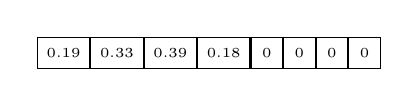
\begin{tikzpicture} [
                    cell/.style={draw, minimum width={4mm}, minimum height={4mm}, solid, thin}
                ]
                \matrix [nodes=draw]
                {
                \node [cell] {\tiny 0.19}; & \node [cell] {\tiny 0.33};   & \node [cell] {\tiny 0.39}; & \node [cell] {\tiny 0.18}; & \node[cell]  {\tiny 0};  & \node[cell]  {\tiny 0}; & \node [cell] {\tiny 0}; & \node [cell] {\tiny 0};\\
            };
                \end{tikzpicture} 
            };
        \end{tikzpicture} 
    };
    
    \draw[edge] (eventTemplates) -- (0, -8) node [midway, fill=white] {\footnotesize \textcolor{customGreen}{feature extraction}};
    

\end{tikzpicture}
   \caption{An example of encoding log sequence into two types of feature vectors: \textit{Event count vector} and \textit{TF-IDF vector}. We assume that there is $8$ event templates in the collection, thus the output vectors are also of length $8$.}
	\label{fig:feature-extraction}
	}
\end{figure}

\begin{table}
\centering
\resizebox{\textwidth}{!}{\begin{tabular}{@{}ccc@{}}
\toprule
\textbf{Matrix type} & \textbf{Row}               & \textbf{Column}                                          \\ \midrule
\textbf{\textcolor{customRed}{Event count}}    & log sequence & Frequency of event type in the log sequence              \\
\textbf{\textcolor{customRed}{TF-IDF}}         & log sequence & IDF weighted frequency of event type in the log sequence \\ \bottomrule
\end{tabular}}
\caption{A summary of feature matrix types using in our thesis }\label{tab:embeddings-summary}
\end{table}

\subsubsection*{Event Count Matrix}
A simple approach to obtain such representation is to create a event count vector for each log sequence. In other words, for each log sequence, we count the number of event type identifiers and store it as a row vector of an event count matrix. The length of the vector corresponds with the number of unique event types detected in the log parsing section, and each component of the vector corresponds to one event type. The value at each position in the vector is the frequency of event types. For event types that did not occur in the log sequence, the value is zero. Thus, one row of the event count matrix represents a single log sequence. The valuable information contributing to the machine learning model behind the event count matrix is determining what is a normal count of events and what does it mean to deviate from the normal counts.

%http://essay.utwente.nl/83142/1/Ma_MA_FacultyOfEEMathematicsAndCS.pdf illustration

This way of constructing the event count matrix is known in the literature as a natural language processing (NLP) model for feature extraction called \textit{Bag-of-Words} (BoW) \cite{informationRetrieval2008}. BoW treats each log sequence as a \textit{document} and for each \textit{word} (in our case, a word is an event type) in a document, a \textit{weight} is assigned. The weight depends on the number of occurrences of the term in the document. The length of the vector corresponds with the number of unique words in the database (analogous to all parsed event types). Then the weight score is referred to as \textit{Term Frequency} (TF) and denoted as $tf_{t,d}$, where the subscript $t$ refers to term (event type) and $d$ refers to document (log sequence) and $f_{t,d}$ is a frequency of term $t$ in document $d$. Term frequency describes the importance of an event type in a log sequence.

\begin{gather}
    tf_{t,d} = \dfrac{f_{t,d}}{\sum_{t'}f_{t', d}}
\end{gather}

In other words, $tf_{t, d}$ is the probability of occurrence of $t$ in $d$.

\subsubsection*{TF-IDF}
Another weighting scheme widely used in Information Retrieval is called \textit{term frequency–inverse document frequency} (TF-IDF). 

Using only the standard term frequency, we have to deal with an important issue. From the definition of term frequency, all event types are considered equally important \cite{informationRetrieval2008}. However, we would also like to know how important a term is not only in one document, but in the whole dataset. That's where another weight score, \textit{inverse document frequency} (IDF) comes to play. First, let us define \textit{document frequency} (DF). Document frequency $df_t$ is defined as the number of documents in the collection that contain the term $t$. Then the inverse document frequency $df_t$ of the term $t$ is defined as: 

\begin{gather}
    idf_t = \log{\dfrac{N}{df_t}}
    \label{formula:idf}
\end{gather}

where $N$ is the total number of documents in the collection. We can observe that if a term is rarely occurring in the collection, the $idf$ is high, and if the term is frequent, then the $idf$ is low.

By the definition, TF-IDF weighting of a term $t$ in document $d$ is a product of two quantities: the term frequency $tf_t$ and the inverse document frequency $idf_t$:

\begin{gather}
    tf\text{-}idf_{t, d} = tf_{t,d} \times idf_t
    \label{formula:tfidf}
\end{gather}

The intuition behind the components of TF-IDF weight is that the term frequency gives higher weight to terms that are frequently occurring in a single document. On the contrary, inverse document frequency gives lower score to words that are frequently occurring in the whole collection, as we are more interested in those that happen rarely. Thus, the $tf\text{-}idf_{t, d}$ weight of the term $t$ in document $d$ is 

\begin{enumerate}
    \item higher, if the term $t$ is frequently occurring in the small number of documents
    \item lower, if the term $t$ is rarely occurring in the high number of documents or if the term $t$ is rarely occurring in the document $d$
    \item lowest, if the term $t$ occurs in all of the document in the collection
\end{enumerate}

As a result, the feature vector of the log sequence is a vector with the value of each dimension defined by \ref{formula:tfidf}.

Final log sequence vectorization contains normalization of IDF weight by scaling between 0 and 1. There are several ways to normalize IDF, but we decided to use a common approach of applying \textit{logistic} (sigmoid) function to normalize IDF:

\begin{align*}
    tf\text{-}idf_{t, d} &= tf_{t,d} \times \sigma(idf_t) \\
    \sigma(x) &= \dfrac{1}{1 + e^{-x}}
\end{align*}

\subsubsection*{TF-IDF example}
We will show an example of how TF-IDF is computed in our case, where we work with log sequences instead of documents and event type identifiers instead of terms. Let's assume we have a collection of log sequences and we extracted $8$ event templates from our dataset. Each log message found in log sequence is marked by its corresponding event type identifier starting from $1$ to $8$, as shown in Table \ref{tab:tfidfexample1}.

\begin{table}
\centering
\begin{tabular}{@{}C{10cm}C{10cm}@{}}
\toprule
\textbf{Log sequence ID} & \textbf{Event Types} \\ \midrule
$l_1$                       & {$[1, 4, 1, 3, 7]$}               \\
$l_2$                         & {$[3, 3, 3, 8, 4]$}               \\
$l_3$                         & {$[2, 7]$}               \\
$l_4$                         & {$[3, 3, 6, 8, 4, 6]$}               \\ \bottomrule
\end{tabular}
\caption{An example of log sequences, which comprises different amounts of log messages. Log message is represented by the event type identifier.}\label{tab:tfidfexample1}
\end{table}

In order to compute the term frequency, we find the frequencies of event types in each log sequence and then normalize the frequencies to get the row vectors sum up to $1$. To continue with our example set of log sequences, the TF score computation is described in Table \ref{tab:tfidfexample2}.

\begin{table}[!h] 
\begin{subtable}[b]{1\textwidth}
\centering
  \begin{tabular}{@{}ccccccccc@{}}
        \toprule
        \backslashbox{Log sequence ID}{Event type ID} & \textbf{1} & \textbf{2} & \textbf{3} & \textbf{4} & \textbf{5} & \textbf{6} & \textbf{7} & \textbf{8} \\ \midrule
        $l_1$                     & 2          & 0          & 1          & 1          & 0          & 0          & 1          & 0          \\ \midrule
        $l_2$                     & 0          & 0          & 3          & 1          & 0          & 0          & 0          & 1          \\ \midrule
        $l_3$                     & 0          & 1          & 0          & 0          & 0          & 0          & 1          & 0          \\ \midrule
        $l_4$                     & 0          & 0          & 2          & 1          & 0          & 2          & 0          & 1          \\ \bottomrule
        \end{tabular}
        
        \caption{Computation of the frequency $f_{t,d}$ of term $t$ in document $d$.}
    \end{subtable} \\
	\hfill
	\\
    \begin{subtable}[b]{1\textwidth}
    \centering
      \resizebox{\textwidth}{!}{\begin{tabular}{@{}ccccccccc@{}}
        \toprule
        \backslashbox{Log sequence ID}{Event type ID} & \textbf{1} & \textbf{2} & \textbf{3} & \textbf{4} & \textbf{5} & \textbf{6} & \textbf{7} & \textbf{8} \\ \midrule
        $l_1$                     & 2/5          & 0          & 1/5          & 1/5          & 0          & 0          & 1/5          & 0          \\ \midrule
        $l_2$                     & 0          & 0          & 3/5          & 1/5          & 0          & 0          & 0          & 1/5          \\ \midrule
        $l_3$                    & 0          & 1/2          & 0          & 0          & 0          & 0          & 1/2          & 0          \\ \midrule
        $l_4$                     & 0          & 0          & 1/3          & 1/6          & 0          & 1/3          & 0          & 1/6          \\ \bottomrule
        \end{tabular}}
        \caption{Computation of the TF score $tf_{t,d} = \dfrac{f_{t,d}}{\sum_{t'}f_{t', d}}$.}
    \end{subtable}%
    \caption{Computation of the TF score.}
	\label{tab:tfidfexample2}
\end{table}

To compute the IDF, we first calculate the document frequency $df_t$ of each term and use the formula \ref{formula:idf} to obtain the inverse document frequencies. We will leave out the normalization for illustration purposes.

\begin{table}[!h] 
\begin{subtable}[b]{1\textwidth}
\centering
  \begin{tabular}{@{}ccccccccc@{}}
        \toprule
        \backslashbox{Log sequence ID}{Event type ID} & \textbf{1} & \textbf{2} & \textbf{3} & \textbf{4} & \textbf{5} & \textbf{6} & \textbf{7} & \textbf{8} \\ \midrule
        \textbf{$l_1$}                     & 2          & 0          & 1          & 1          & 0          & 0          & 1          & 0          \\ \midrule
        \textbf{$l_2$}                     & 0          & 0          & 3          & 1          & 0          & 0          & 0          & 1          \\ \midrule
        \textbf{$l_3$}                     & 0          & 1          & 0          & 0          & 0          & 0          & 1          & 0          \\ \midrule
        \textbf{$l_4$}                     & 0          & 0          & 2          & 1          & 0          & 2          & 0          & 1 \\ \midrule
        $\mathbf{n_t}$                  & 1          & 1          & 3          & 3          & 0          & 1          & 2          & 2         
        \\ \bottomrule
        \end{tabular}
        
        \caption{Computation of the document frequency $df_{t}$ of term $t$.}
    \end{subtable} \\
	\hfill
	\\
    \begin{subtable}[b]{1\textwidth}
    \centering
      \resizebox{\textwidth}{!}{\begin{tabular}{@{}ccccccccc@{}}
        \toprule
        \backslashbox{Log sequence ID}{Event type ID} & \textbf{1} & \textbf{2} & \textbf{3} & \textbf{4} & \textbf{5} & \textbf{6} & \textbf{7} & \textbf{8} \\ \midrule
        \textbf{$l_1$}                     & 0.602          & 0,602          & 0.125          & 0.125          & 0          & 0.602          & 0.301          & 0.301         \\ \bottomrule
        \end{tabular}}
        \caption{Computation of the IDF score $idf_t = \log{\dfrac{N}{df_t}}$. In our example, $N=4$ as there are $4$ log sequences in the collection. For instance, IDF weight of the event type $1$ is calculated as $idf_1 = \log{\dfrac{4}{1}} = 0,602$.}
    \end{subtable}%
    \caption{Computation of the IDF score.}
	\label{tab:tfidfexample3}
\end{table}

The final step is calculating the product $TF \times IDF$ and the values are shown in Table \ref{tab:tfidfexample4}.

\begin{table}[!h]
    \centering
    \resizebox{\textwidth}{!}{\begin{tabular}{@{}ccccccccc@{}}
        \toprule
        \backslashbox{Log sequence ID}{Event type ID} & \textbf{1} & \textbf{2} & \textbf{3} & \textbf{4} & \textbf{5} & \textbf{6} & \textbf{7} & \textbf{8} \\ \midrule
        \textbf{$l_1$}                     & 0.2408          & 0          & 0.025          & 0.025          & 0          & 0          & 0.0602          & 0          \\ \midrule
        \textbf{$l_2$}                     & 0          & 0          & 0.075          & 0.025          & 0          & 0          & 0          & 0.0602          \\ \midrule
        \textbf{$l_3$}                     & 0          & 0.301          & 0          & 0          & 0          & 0          & 0.1501          & 0          \\ \midrule
        \textbf{$l_4$}                     & 0          & 0          & 0.042          & 0.021          & 0          & 0.201          & 0          & 0.05
        \\ \bottomrule
        \end{tabular}}
    \caption{TF and IDF scores from the example are multiplied to obtain TF-IDF}.
    \label{tab:tfidfexample4}
\end{table}

We assume that by using TF-IDF weighting, we will provide an extra information about the event type distribution not only in terms of log sequences, but also in the whole data set, that could potentially increase ML model's performance. 

\section{Anomaly Detection}

Now that we have created the feature matrices, machine learning methods can be applied to detect outliers in the data. For our experiments, we are using an open-source machine learning toolkit \textit{Loglizer}. 

\subsection{Loglizer}
\label{subscetion:loglizer}

Loglizer\footnote{https://github.com/logpai/loglizer} is an open-source machine learning based log analysis toolkit for automated anomaly detection written in Python \cite{he2016}. Loglizer was developed for automated anomaly detection as a part of LogPAI \footnote{\url{http://www.logpai.com}}, which is a collection of AI-based log analytics solutions. These log analysis tools have been used by industrial teams in Microsoft and Huawei. It includes three supervised anomaly detection models (\textit{Logistic Regression, Decision Tree, Support Vector Machine}) and six unsupervised anomaly detection models (\textit{Local Outlier Factor, One-Class SVM, Isolation Forest, Principal Component Analysis, Invariants Mining, Clustering}). At the time of writing this thesis, another two unsupervised models were in the development (\textit{DeepLog, AutoEncoder}). 

We decided to leverage a third-party toolkit for several reason. Firstly, as the algorithms we are using in our experiments have been already implemented, there is no need to completely reinvent the wheel and write the implementation ourselves. This way we can avoid a time consuming process and rather focus on the main intention of our research - to investigate if applying various anomaly detection techniques on a real-world dataset can lead to successful results and how to approach it.

Another benefit is that the Loglizer anomaly detectors are working with log sequences. This means that each of the models is trained on a set of log sequences, and the output of the detector classifies whether a single log sequence is an anomaly or not. As described in Section \ref{section:featureEngineering}, we use windowing for generating the log sequences, which makes the Loglizer toolkit a great fit in our research context. Specifically, four methods were used in our research: Invariants Mining, Isolation Forest and PCA. The underlying algorithms behind these tools are presented in Section \ref{section:anomalyDetectionLiteratureReview}.

Implemented anomaly detection methods are evaluated on a public dataset, HDFS. Logs in HDFS dataset were collected from Amazon EC2 platform and contain $11\,175\,629$ entries \cite{xu2009}. Loglizer provides benchmarking results on both supervised and unsupervised methods separately using this dataset, which can be found in Table \ref{table:loglizer}. Evaluation metrics are explained in Section \ref{section:evaluationMetrics}. Benchmarking gives a better idea of the expected performance of the anomaly detection methods we are planning to use in our work. 

Last but not least, Loglizer makes it easier to reproduce, understand and customize the experiments, as the code is open-source.

\begin{table}[h]
\centering
\begin{tabular}{@{}cccc@{}}
\toprule
\multicolumn{4}{c}{\textbf{HDFS}} \\ 
\textbf{Model}    & \textbf{Precision} & \textbf{Recall} & \textbf{F1} \\  \toprule \midrule
\multicolumn{4}{c}{\textit{Supervised Methods}}                        \\ \midrule
LR                & 0.955              & 0.911           & 0.933       \\
Decision Tree     & 0.998              & 0.998           & 0.998       \\
SVM               & 0.959              & 0.970           & 0.965       \\ \midrule
\multicolumn{4}{c}{\textit{Unsupervised Methods}}                      \\ \midrule
LOF      & 0.967              & 0.561           & 0.710       \\
One-Class SVM     & 0.995              & 0.222           & 0.363       \\
Isolation Forest  & 0.830              & 0.776           & 0.802       \\
PCA               & 0.975              & 0.635           & 0.769       \\
Invariants Mining & 0.888              & 0.945           & 0.915       \\
Clustering        & 1.000              & 0.720           & 0.837       \\ \bottomrule
\end{tabular}
\caption{Benchmarking results of three supervised and six unsupervised anomaly detection methods on HDFS dataset \cite{he2016}}.
\label{table:loglizer}
\end{table}

\subsection{Experiment Workflow}
Running machine learning experiments is usually an iterative process, where each iteration requires different configuration parameters, input training and testing datasets and a lot of file handling. The same holds for our anomaly detection experiments. We obtained several raw datasets from the SmartConnect's system. We picked four anomaly detection methods, where each method might require a different dataset as well as its own parameter configuration. Every raw dataset needs to parsed from its initial JSON file into a unified structure, it needs to be cleaned and faulty log entries need to be removed. Then a log parser program is applied to obtain an event type identifier for each log message. Finally, we use two different feature matrix representations as an input for anomaly detection methods. After having obtained trained models for every dataset, the evaluation follows. Having so many dependent processes to perform for each experiment iteration where things can get messy very easily, makes it desirable to have an automated workflow system. Despite our thesis not being a software engineering thesis, thus the focus was not on having a perfectly extensible workflow, we attempted to come up with a solution that saves time required to run experiments.

We created a Makefile-based pipeline comprising a set of Python scripts to facilitate experiments. The goal was to have a reproducible, modular and scalable solution to deal with the complexity of conducting experiments. In this section, we will briefly describe the architecture of this pipeline and the implementation of the experiment scripts.
 
 \subsubsection*{Makefile}
The experiment execution is orchestrated by the GNU \textit{make} instructions described in the Makefile scripts. A Makefile consists of a set of rules that generate target files if any of their dependencies change. We decided to use Makefile because it directly enforces a modular character to our workflow. Every rule must follow the shape:

\begin{verbatim}
    target ... : prerequisities ... 
        recipe
        ...
\end{verbatim}

 Usually, targets and prerequisities are file names and recipes are commands. Makefile can be expressed by a directed acyclic dependency graph \cite{feldman1979make}. The dependency graph of our Makefile is illustrated in Figure \ref{fig:makefile}. 
 
 Each target contained in the Makefile operates on the \texttt{DATASET} variable assignment. \texttt{DATASET} represents the name of the dataset, that needs to exist in the \texttt{data/raw/} directory of the project folder before any of the targets are run, therefore we call it a \textit{prerequisity} or a \textit{dependency}. The variable can be set from outside of the Makefile as part of the command line. Changing the value of \texttt{DATASET} directly influences the names of the generated output files. By running \texttt{make} in the directory containing Makefile and assigning \texttt{DATASET} variable, we can manage the experiment workflow:
 
 \begin{itemize}
     \item \texttt{make} \textit{data} \texttt{DATASET=<dataset name>}
     \begin{itemize}
         \item Parses JSON file with raw data into a panda's DataFrame
         \item Flattens columns of the DataFrame that contain nested JSON structures
         \item Executes log abstraction by processing log messages, extracting an event type for each log message and appending event type column to the DataFrame
         \item Stores DataFrame with preprocessed logs 
         \item Extracts event count and TF-IDF feature matrices
         \item Stores feature matrices
     \end{itemize}
     \item \texttt{make} \textit{train} \texttt{DATASET=<dataset name>}
     \begin{itemize}
         \item Executes training script and generates invariant mining, isolation forest, log clustering and PCA models using event count and TF-IDF feature matrices
         \item Stores models
     \end{itemize}
     \item \texttt{make} \textit{evaluate} \texttt{DATASET=<dataset name>}
     \begin{itemize}
         \item Executes evaluation script for invariant mining, isolation forest, log clustering and PCA models trained using event count and TF-IDF feature matrices by detecting anomalies on provided labeled dataset
         \item Generates precision, recall and F1 score into CSV files stored in \texttt{\justify results/metrics} directory
         \item Generates labels predicted by all the models into CSV files stored in~\texttt{results/predictions} directory
     \end{itemize}
     \item \texttt{make} \textit{all} 
     \begin{itemize}
         \item Runs all modules of the workflow
     \end{itemize}
     \item \texttt{make} \textit{clean} \texttt{DATASET=<dataset name>}
     \begin{itemize}
         \item Cleans up all generated files related to \texttt{DATASET} including the trained model, if it exists
     \end{itemize}
 \end{itemize}
 
 \begin{figure}[!h] \centering {
   \begin{tikzpicture} [
    edge/.style={-latex,shorten >=1pt, thin, color=customGrey},
    line/.style={-,shorten >=1pt, thin, color=customGrey},
    fileTarget/.style={rectangle, draw=customBlue, align=left, minimum width=55mm, minimum height=7mm},
    phonyTarget/.style={rectangle, draw=customRed, align=left, minimum width=20mm, minimum height=7mm}
]

\node[fileTarget, align=center] (root) at (0, 0) {\tiny data/raw/\$(DATASET).json};

\node[fileTarget, align=center] (preprocessed_tf) at (-3, -1.5) {\tiny data/preprocessed/tf/\%-preprocessed.pickle};

\node[fileTarget, align=center] (preprocessed_tfidf) at (3, -1.5) {\tiny data/preprocessed/tfidf/\%-preprocessed.pickle};

\draw[edge] (root) -- (preprocessed_tf);
\draw[edge] (root) -- (preprocessed_tfidf);

\node[fileTarget, align=center] (features_tf) at (-3, -3) {\tiny data/features/tf/\%.npy};

\node[fileTarget, align=center] (features_tfidf) at (3, -3) {\tiny data/features/tfidf/\%.npy};

\draw[edge] (preprocessed_tf) -- (features_tf);
\draw[edge] (preprocessed_tfidf) -- (features_tfidf);

\node[phonyTarget, align=center] (data) at (0, -4.5) {\tiny data};

\draw[edge] (features_tf) -- (data);
\draw[edge] (features_tfidf) -- (data);

\node[fileTarget, align=center] (model_tf) at (-3, -6) {\tiny models/tf/\%.model};

\node[fileTarget, align=center] (model_tfidf) at (3, -6) {\tiny models/tfidf/\%.model};

\draw[edge] (features_tf) -- (model_tf);
\draw[edge] (features_tfidf) -- (model_tfidf);

\node[phonyTarget, align=center] (train) at (0, -7.5) {\tiny train};

\draw[edge] (model_tf) -- (train);
\draw[edge] (model_tfidf) -- (train);

\node[fileTarget, align=center] (results) at (0, -9) {\tiny results/\%.csv};

\draw[edge] (model_tf) -- (results);
\draw[edge] (model_tfidf) -- (results);

\node[phonyTarget, align=center] (evaluate) at (0, -10.5) {\tiny evaluate};

\draw[edge] (results) -- (evaluate);

\node[phonyTarget, align=center] (all) at (0, -12) {\tiny all};

\draw[edge] (evaluate) -- (all);

\end{tikzpicture}
   \caption{A dependency graph for a Makefile to run experiments in our thesis. Blue rectangles represent the \textit{file targets} and the red rectangles represent \textit{phony targets}. Phony targets are are targets that are not creating or updating a file, but they represent a name for a sequence of commands to be executed. Phony targets allow our experiments to be executed in a modular manner.}
	\label{fig:makefile}
	}
\end{figure}

Models and their configurations, that will be trained in the pipeline, can e specified from inside of the Makefile.

\subsubsection*{Scripts Implementation}
 Having a consistent file naming convention and a consistent file organization into directories and subdirectories is crucial for automated experiments. The example of our experiment directory structure that is designed for use with Makefile is in the Appendix \ref{appendix:dir_structure}.
 
 Each machine learning method has three Python scripts in the \texttt{src/models} directory: \textit{train}, \textit{evaluate} and the \textit{model} itself. 
 
 Each \textit{model} script functions as a wrapper with a common interface, that contains algorithm providing library (in our case, we are using LogLizer library, as described in Section \ref{subscetion:loglizer}) and enables calling the following methods:
 
\begin{itemize}
    \item \texttt{\_\_init\_\_}
    \item \texttt{fit}
    \item \texttt{predict}
    \item \texttt{evaluate}
    \item \texttt{save}
    \item \texttt{load}
\end{itemize}

The advantage of having a wrapper above the actual model is that it can be easily replaced by other library providing the model implementation, or we can provide our own implementation.

As one can see from the list above, each model also contains \texttt{save} and \texttt{load} methods. They are included in the model as a mean of serialization and deserialization of the trained model. The reason for that is the fact that training a model is usually a very time consuming task. Being able to load an already trained model saves us the trouble of training the model every time it is required. A serialized model can be conveniently restored later and used for evaluation or prediction. We use \texttt{pickle}\footnote{https://docs.python.org/3/library/pickle.html} library, that converts arbitrary Python's object into a byte stream. The process of serializing the data is then referred to as "pickling" and deserializing as "unpickling".

\textit{Train} scripts allow optional and model-specific parameters to tune the models. These parameters can be modified in the Makefile. Then they simply load the preprocessed data, instantiate the model and execute the model training process. Finally, the trained model is stored into a pickle. 
 
\textit{Evaluate} scripts contain loading the trained model and running the \texttt{\justify evaluate} method to obtain metrics and predictions.

As shown in the directory structure in the Appendix \ref{appendix:dir_structure}, preprocessed features, trained models and resulting metrics and predictions are stored in either \texttt{tf} or \texttt{tfidf} folder, depending to which feature extraction method the particular file belongs. \texttt{tf}, as an abbreviation for term frequency, is an equivalent of what we call in our thesis an \texttt{event count}, as we explained in detail in Section \ref{subsection:features}. We use \texttt{tf} in our file structure for the benefit of brevity.

\subsection{Mapping from Prediction Back to Log Entry}
Once the output is computed, what we obtain is a prediction for each window of the input dataset. This is true regardless of the specific machine learning model used for the computation. 
This kind of output that consists from ones and zeros is not very helpful if we want to understand why we got those results and if they are correct. Ideally, we want more elaborate information about the individual windows.
Typically, the interesting part would be those windows, that were identified as anomalous as they are assumed to be less frequent and more important. However, there are use cases where we want to investigate all of them, especially in the debugging phase. 

From a feature vector of a given window, only event type's ID and frequency is stated, the template and order is lost.
After discussing with domain experts what would be a valuable information about a time window, we concluded that with every window it should be also provided:
\begin{itemize}
    \item \textit{How frequent is each of the event types and what is the template of each event.}\\
    We create a histogram, ordered descending from the most frequent events to the least frequent. This gives a good overview of what is the state of the system in a given time window. 
    \item \textit{Raw trace of logs within the window.}\\
    Histogram is a good start but for some cases, details and preserved order matter. In some cases also the variable parts of log messages that are missing in the log templates need to be known to gain a clear picture of what was going on in the system. Therefore, we also assign trace of raw logs ordered by the time as they happened.
    \item \textit{What time range a window corresponds to.}\\
    It is simple to map from a window index to human readable time. This way, an expert can tell whether something special was happening in the system. For example, regular testing may take place at specific times everyday, which can explain some behaviour.
\end{itemize}
 
% Flowchart: https://bost.ocks.org/mike/make/

